

\documentclass[12pt]{article}
   
   \usepackage[utf8]{inputenc}
   \usepackage{graphicx}
   \usepackage{float}
   \usepackage{subcaption}
   %\usepackage{mathtools}
   \usepackage{amsmath}
   
   \addtolength{\hoffset}{-0.7in}
   \addtolength{\textheight}{1.5in}
   \addtolength{\textwidth}{1.5in}
   \addtolength{\voffset}{-1in}
 
\title{ EE230: Experiment 2 \\
       Non-idealities in Op-amps}
       
\author{karthikgvb }
\date{January 2020}


%_____________________________________________________________________________________


\begin{document}
   
   \maketitle

   \section{Overview of the Experiment}
      
      \subsection{Aim of the experiment}
      
      \hspace{2cm} In this experiment we looked into the bad side of an op-amp i.e the problems/errors one might come across under using an op-amp caused by its non-ideal characteristics, we analysed three different non-ideal properties of the UA 741 op-amp 
      \vspace{0.3cm}
      \\ a) Input Offset voltage \\ b) Input Bias currents \\ c) Finite open-loop gain \\
      
      Non-idealities occur because the transistors in the op amp (see Fig. 1) such as Q1 and Q2 which are supposed to be identical, always have some small difference between them in reality, e.g., their $\beta$ values could be slightly different.
      

      
      \subsection{Methods}
      
        \begin{itemize}
           
           \item For measuring offset voltage and bias currents, we enhanced the contributions of one of these parameters while keeping the other two contibutions small by using special circuits.
           
           \item Measurement of the DC open loop gain is achieved by using high closed loop gain non-inverting amplifier so that open loop gain contributes to the actual gain of the amplifier.
           
           \item We also measured open loop gain of AC input signal for different frequencies to understand a brief relation of open loop gain with frequency. 
           
        \end{itemize}
      
    \section{Design of Op-amp 741}
    
        \begin{figure}[H]
            \centering
            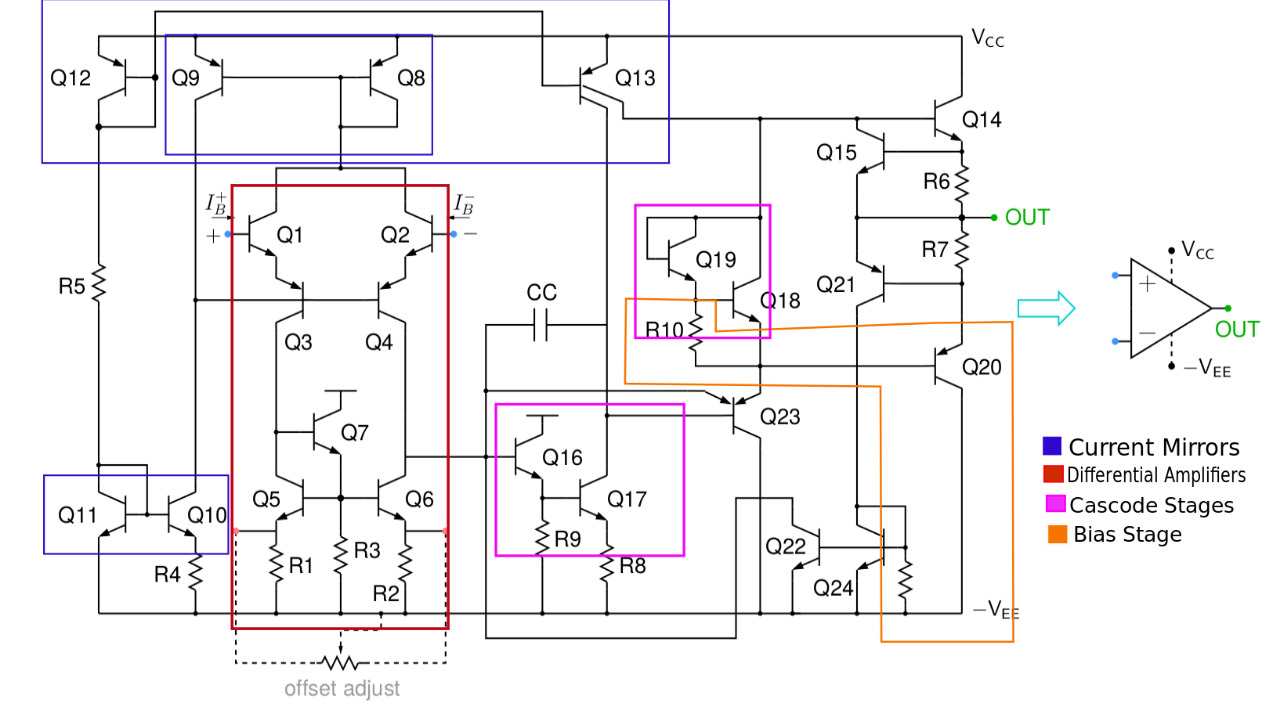
\includegraphics[width = \linewidth]{LAB-1/opamp.jpeg}
            \caption{Internal circuit of Op Amp 741}
        \end{figure}
        
        \begin{figure}[H]
            \centering
            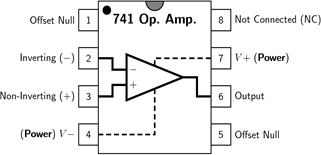
\includegraphics[width = \linewidth, height = 2in]{LAB-1/PinConfig.png}
            \caption{Pinout of Op Amp 741}
        \end{figure}
        
        \newpage       
%________________________________________________________________________________________    
    \section{Experimental results}
    
      \subsection{Input offset voltage measurement} 
        \begin{figure}[H]
            \centering
            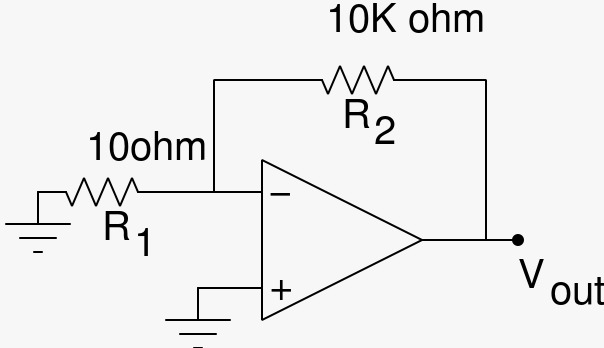
\includegraphics[width = 0.6\linewidth, height = 2in]{LAB-1/offset.jpeg}
            \caption{Circuit to measure Offset voltage}
        \end{figure}
        
        \begin{figure}[H]
            \centering
            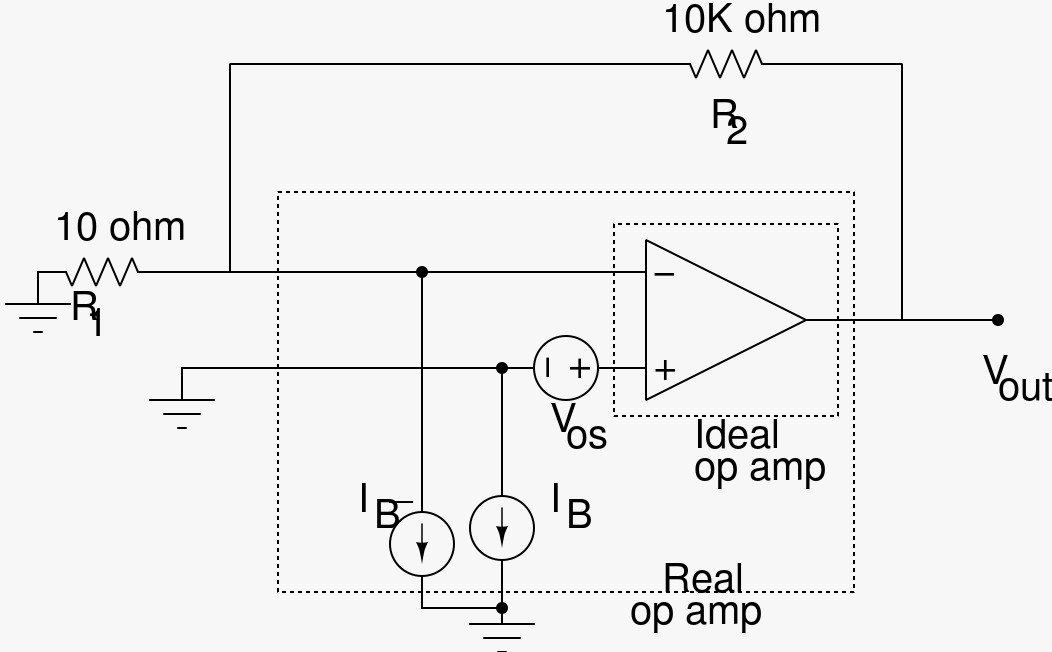
\includegraphics[width = 0.8\linewidth, height = 2.5in]{LAB-1/offset_real.jpeg}
            \caption{Internal Circuit to measure Offset voltage}
        \end{figure}
        
        \begin{equation}
            V_0 = V_{OS}\left(1 + \frac{R_2}{R_1}\right) + R_2I^-_B 
        \end{equation}
      
        By choosing $R_2 \ and \ R_1$ as given in the circuit, we can neglect the second term in the above equation as $V_{OS} \approx 5mV$ and $I_B \approx 100nA$. \\
        Hence
        \begin{equation}
            V_{OS} = \frac{V_0}{1 + \frac{R_2}{R_1}}  
        \end{equation}
        
        The observed output value for $ua 741$ is  $1.11V$, hence \begin{equation}
            \boxed{\mathbf{V_{OS} = 1.11mV}}
        \end{equation}
      
      \subsection{Bias currents measurement}
        \begin{figure}[H]
            \centering
            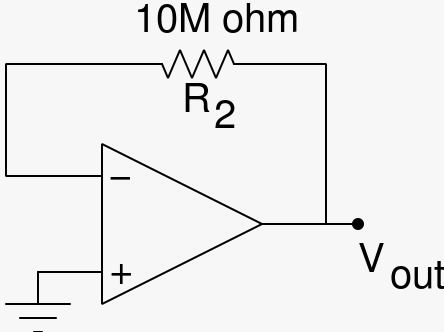
\includegraphics[width = 0.5\linewidth, height = 1.8in]{LAB-1/ibminus.jpeg}
            \caption{Circuit to measure $I^-_B$}
        \end{figure}
        \begin{figure}[H]
            \centering
            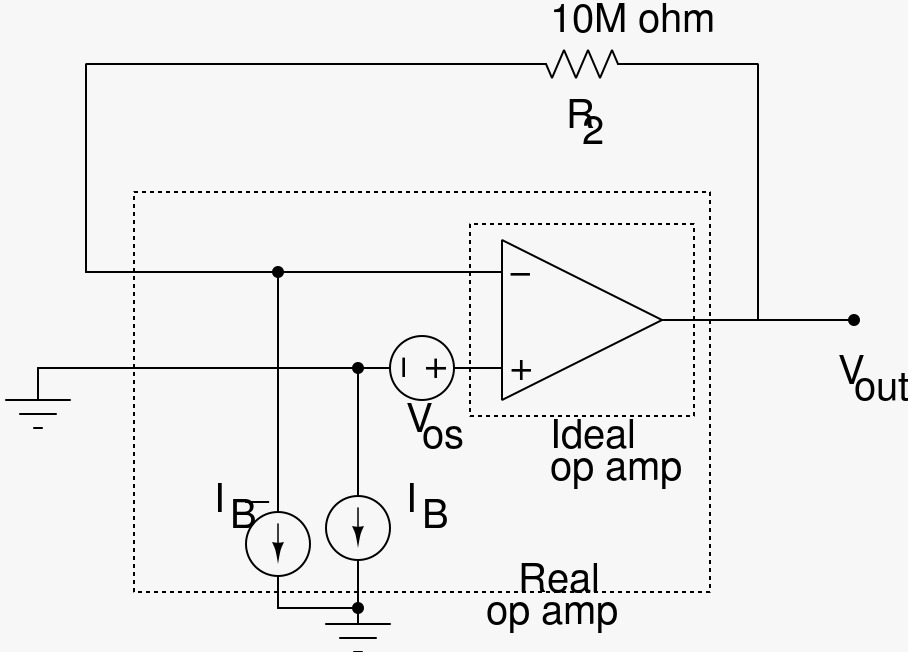
\includegraphics[width = 0.8\linewidth, height = 2.7in]{LAB-1/ibminusreal.jpeg}
            \caption{Internal Circuit to measure $I^-_B$}
        \end{figure}
        \begin{equation}
            V_0 = V_{OS} + RI^-_B
        \end{equation}
        
        R has chosen large so that the second term is large enough to neglect the first term, hence
        
        \begin{equation}
            I^-_B = \frac{V_0}{R}
        \end{equation}
        
        The observed output value for $ua 741$ is  $0.354V$, hence \begin{equation}
            \boxed{\mathbf{I^-_B = 35.4nA}}
        \end{equation}
        
        \begin{figure}[H]
            \centering
            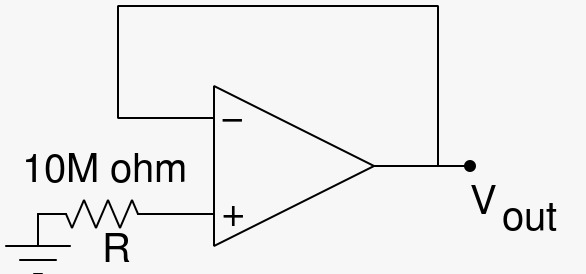
\includegraphics[width = 0.6\linewidth, height = 2in]{LAB-1/ibplus.jpeg}
            \caption{Circuit to measure $I^+_B$}
        \end{figure}
        \begin{figure}[H]
            \centering
            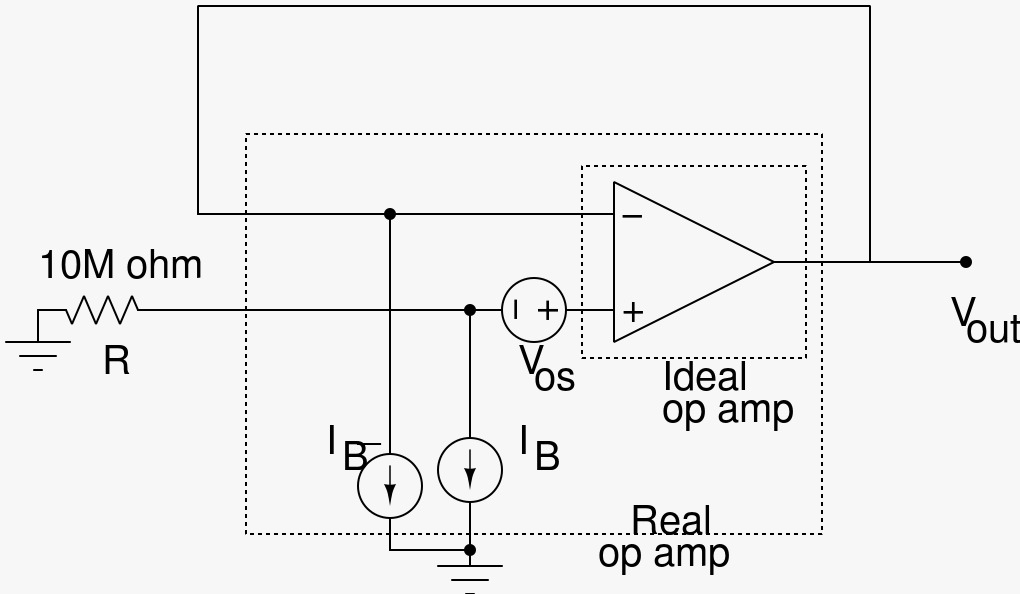
\includegraphics[width = 0.8\linewidth, height = 2.8in]{LAB-1/ibplusreal.jpeg}
            \caption{Internal Circuit to measure $I^+_B$}
        \end{figure}
        \begin{equation}
            V_0 = V_{OS} - RI^+_B
        \end{equation}
        
        Similarly the equation can be approximated to 
        
        \begin{equation}
            I^+_B = -\frac{V_0}{R}
        \end{equation}
        
        The observed output value for $ua 741$ is  $-0.343V$, hence \begin{equation}
            \boxed{\mathbf{I^+_B = 34.3nA}}
        \end{equation}
      
      \subsection{DC open-loop gain measurement}
      
        \begin{figure}[H]
            \centering
            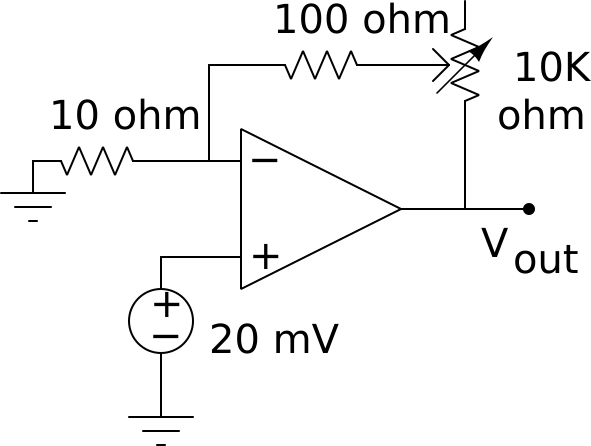
\includegraphics[width = 0.6\linewidth, height = 2.8in]{LAB-1/XC24827.png}
            \caption{Circuit to measure DC open loop gain}
        \end{figure}
        \begin{equation}
            V_0 = V_{OS} - RI^+_B
        \end{equation}
      The actual gain expression for the above circuit is
      \begin{equation}
          Gain = \left(1 + \frac{R_2}{R_1}\right)\frac{1}{1 + \left(1 + \frac{R_2}{R_1}\right)\frac{1}{A_v}} 
      \end{equation}
      
      To find the open loop gain($A_v$), we found the gain for large values of $\left(1 + \frac{R_2}{R_1}\right)$ so that $A_v$ contributes for the actual gain \\
      Also we have taken care of choosing $\left(1 + \frac{R_2}{R_1}\right)$ so that op-amp does not saturate and the actual gain can be measured \\
      
      For $1 + \frac{R_2}{R_1} = 870$ we observed a gain of 663.5 and so $\mathbf{A_v}$ was $\mathbf{2.8\times10^3}$    \\
      
      The challenge we faced in this experiment was finding the feedback resistance as it's a variable resistance, we had to find out the current and the voltage through and across the feedback resistor to find it's resistance along with the output voltage to find the gain. So we ended up with using all the multimeters we have.\\
      
      \textbf{Note:} Instead of nullyfying offset voltage in this experiment using pin 1 and pin 5 of the IC, we included it in the Gain expression. The Gain was adapted to 
      
      \begin{equation}
          Gain = \frac{V_{out}}{V_{in} + V_{OS}}
      \end{equation}
       
      \subsection{Variation of open-loop gain with frequency}
        \begin{figure}[H]
            \centering
            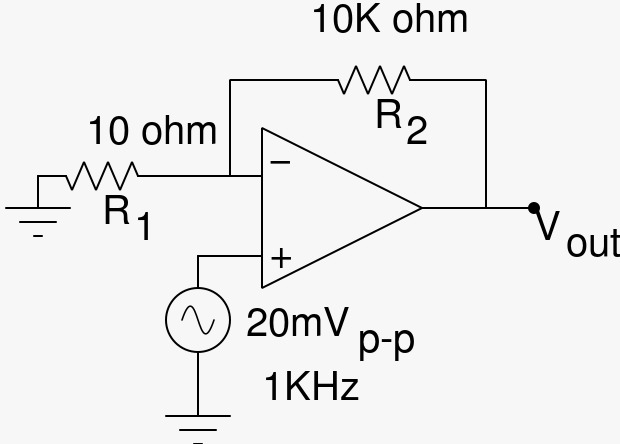
\includegraphics[width = 0.5\linewidth, height = 2in]{LAB-1/olg.jpeg}
            \caption{Circuit to analyse open loop gain with frequency}
        \end{figure}
        \begin{figure}[H]
          \centering
          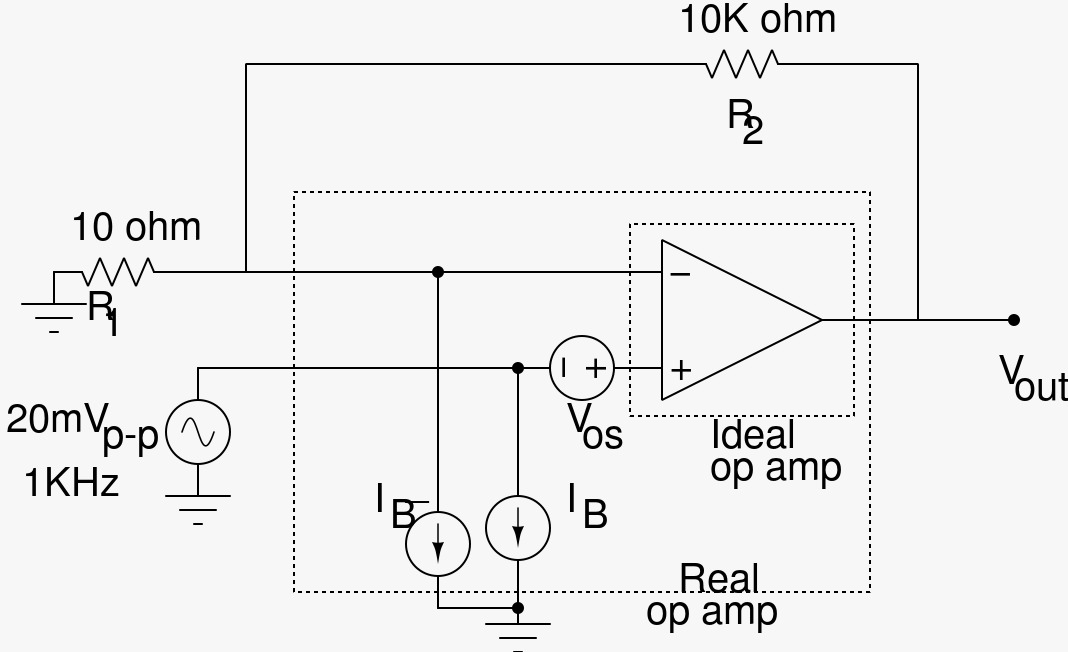
\includegraphics[width = 0.8\linewidth, height = 2.7in]{LAB-1/olgreal.jpeg}
            \caption{Internal circuit of Op Amp 741}
        \end{figure}
      Analysis of open-loop gain with frequency was achieved with AC input which is similar to the previous section with just a change in values of $R_2 = 10K\Omega$ and $R_1 = 10\Omega$ here the closed loop gain was $1000$, the observations were
        
        \begin{figure}[H]
        
            \begin{subfigure}{0.75\linewidth}
                \centering
                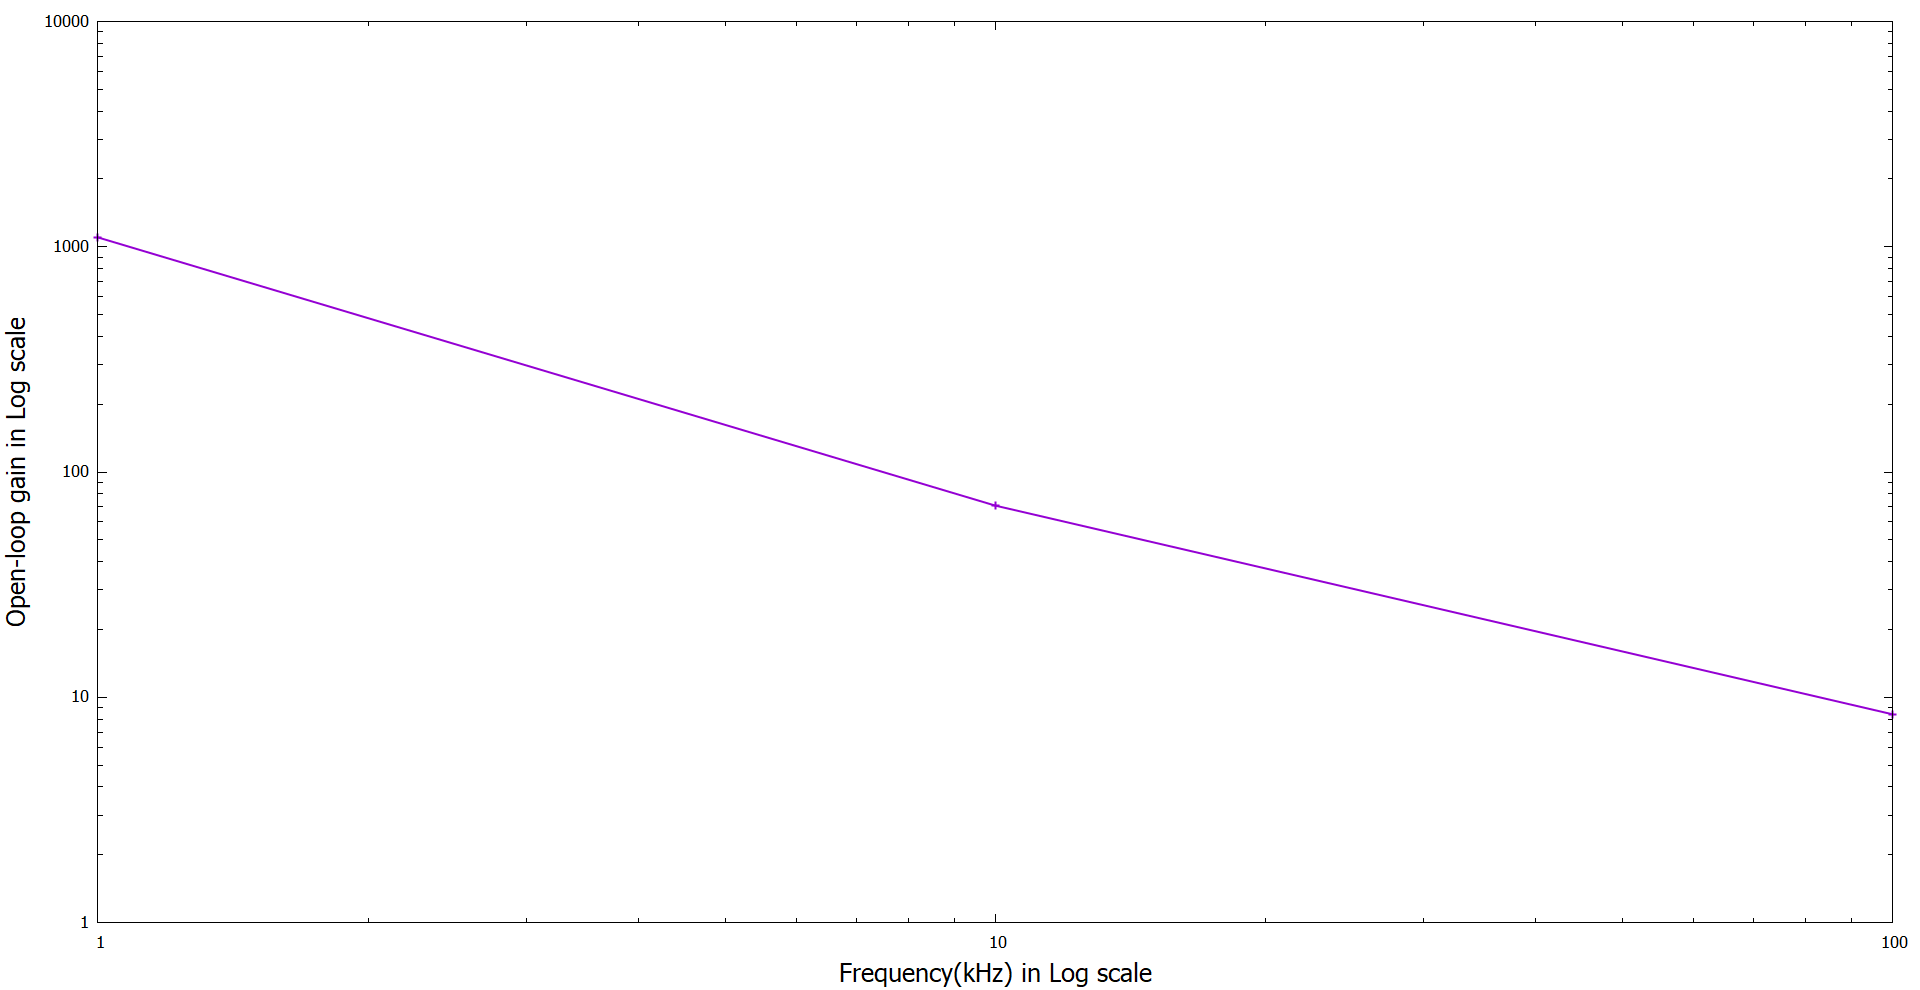
\includegraphics[width = \linewidth]{LAB-1/aLAB-2-1.png}
                \caption{$A_v$ Vs frequency in log scale}
            \end{subfigure}
            \begin{subfigure}{0.1\linewidth}
                \centering
                \begin{tabular}{|c|c|}
                   \hline
                     \bfseries frequency(kHz) & $\mathbf{A_v}$ \\ \hline
                     1  & 1100 \\ \hline
                     10  & 70.93 \\ \hline
                     100  & 8.4 \\ \hline
                \end{tabular}
            \end{subfigure}
        \end{figure}
        
         This plot is linear and matches approximately with the open-loop gain vs frequency curve in log scale given in the datasheet of UA741.
        \begin{figure}[H]
            \centering
            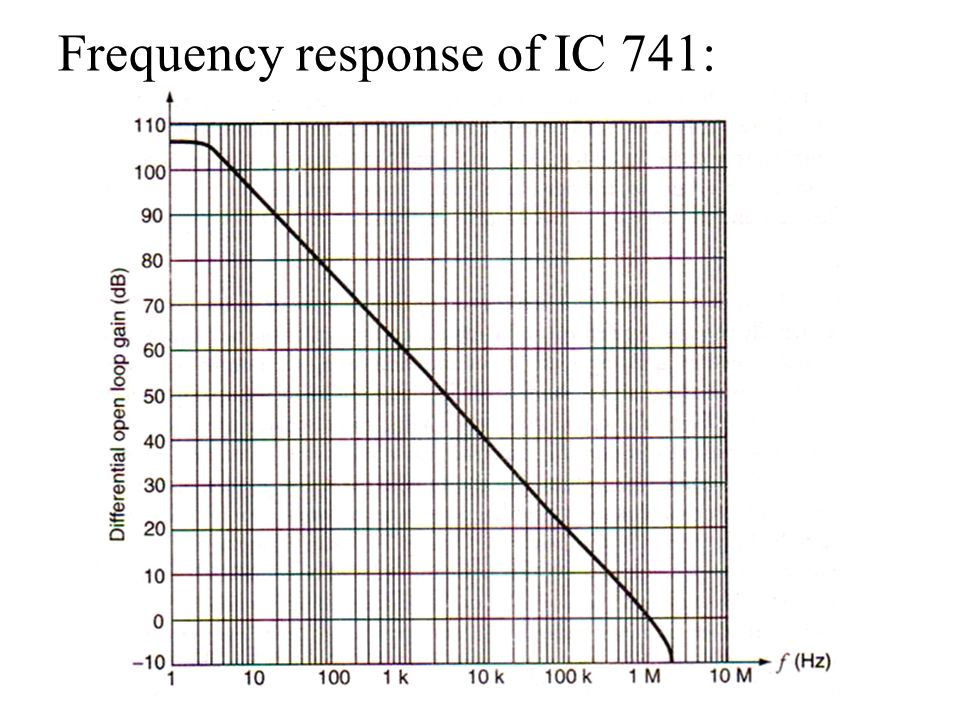
\includegraphics[width = 0.8\linewidth, height = 3in]{LAB-1/slide_14.jpg}
            \caption{Internal circuit of Op Amp 741}
        \end{figure}
        
        \newpage
    
%_________________________________________________________________________________________

    \section{Questions for reflection}  
    
        \begin{itemize}
            \item If the method for null-adjustment is as simple as the one you performed
            in lab, why isn't the 741 op-amp sold with the offset voltage internally calibrated? \\
            
            \textbf{Ans} There could be three reasons:
            \begin{itemize}
                \item The resistance of the pot to be connected to nullify the offset voltage might depend on temperature, supply voltage etc
                \item The offset voltage might be useful for some purposes 
                \item For us to understand the non-idealities of op-amps in the LAB, the 741 op-amp comes without any internal calibration  
            \end{itemize}
            
            \item If the temperature in the lab were different from what it was when you performed the experiment, do you expect the pot value you ended up with will still give you offset nullification? Explain your answer. Hint: Look at the internal circuit diagram and figure out what parameters may change when the temperature changes.
            
            \textbf{Ans} If  the  temperature  in  the  lab  were  different  from  what  it  was  when performed the experiment, the pot value to nullify offset voltage would be different.
            
            \item What is the slew-rate of an op-amp? Read up the definition and explain it in your own words here. Could you suggest an experiment to measure slew-rate of op-amp 741?
            
            \textbf{Ans} The output voltage of an op-amp cannot change instantaneously to any value, it is limited to a rate and the maximum rate at which the output voltage can change is called as slew rate of the op-amp.\\
            
            We can use a non-inverting amplifier of gain one and give a square wave as input, as a square wave is discontinuous we expect the output to change it's value in infinitesimal time which is not observed practically because of slew rate. So the slew rate would be voltage of the top level of the distorted square output voltage signal divided by time taken to reach that level from bottom level. 
            
            \item  What is the role of capacitor C in the circuit you used in the second part of the lab (i.e. in fiigure 8 of the hand-out)? (Hint: there is a statement in the hand-out mentioning why C is connected; could you explain why that statement is true?)
        \end{itemize}
        
        \newpage
        
        \vspace*{5cm}
    \begin{thebibliography}{9}

        \bibitem{Analog LAB Manual} 
        Non-idealities of op-amp File 
        \\\texttt{https://moodle.iitb.ac.in/mod/resource/view.php?id=92663}
        \bibitem{Datasheet of UA741}
        Datasheet of OpAmp UA741
        \\\texttt{https://www.slideshare.net/YongHeuiCho/u-a741}
        
    \end{thebibliography}
     
  
\end{document}